%
% 1dim.tex -- XXX
%
% (c) 2019 Prof Dr Andreas Mueller
%
\section{Das eindimensionale Problem}
\rhead{Der eindimensionale Fall}
Zum Beweis, dass das im vorangegangenen Abschnitt angedeutete Programm 
tatsächlich durchführbar ist,
betrachten wird das eindimensionale Problem
\[
u''(x)=f(x)
\]
mit der Randbedingung
\[
u(0)=a,\quad u(1)=b.
\]
Ziel ist, die Funktion $G$ zu finden.

Die Lösung dieses Problems wird in der Theorie der gewöhnlichen
%\marginpar{\tiny Lösung des gewöhnlichen Randwertproblems als Leitlinie
%für den mehrdimensionalen Fall}
Differential\-gleichungen behandelt, wir wollen hier die allgemeine
Lösung jedoch so darstellen, dass sie als Leitlinie für die
Entwicklung einer Lösung für das mehrdimensionale Problem dienen
kann.
\subsection{Partikuläre Lösung}
Ein Lösung der Gleichung kann sofort gefunden werden, die Stammfunktion
liefert die Lösung
\begin{align*}
u_p'(x)&=\int_0^xf(\xi)\,d\xi,
\\
u_p(x)&=\int_0^xu_p'(\eta)\,d\eta=\int_0^x\int_0^\eta f(\xi)\,d\xi\,d\eta
\end{align*}
diese erfüllt aber die Randbedingung nicht.
Die gesuchte Lösung muss aber eine Summe der partikulären Lösung 
und einer Lösung der homogenen Gleichung
\[
u_p''(x) + u_h''(x)=f(x)\quad\Rightarrow\quad u_h''(x)=0
\]
sein, mit der Randbedingungen
\begin{align*}
u_h(0)&=a-u_p(0)=a\\
u_h(1)&=b-u_p(1)=b-\int_0^1\int_0^\eta f(\xi)\,d\xi\,d\eta
\end{align*}

\subsection{Das homogene Problem}
Das homogene Problem
\[
u''(x)=0
\]
kann mit den Standardverfahren gelöst werden. Die allgemeine
Lösung hat die Form $Ax+B$, die Konstanten müssen so gewählt werden,
dass die Randbedingungen erfüllt sind, also
\begin{align*}
A\cdot 0+B&=a\qquad\Rightarrow&B&=a\\
A\cdot 1+B&=b\qquad\Rightarrow&A&=b-a
\end{align*}
also $u(x)=(b-a)x+a=(1-x)a+xb$.

\subsection{Allgemeine Lösung}
Im vorliegenden Fall sollte $u_h$ den rechten Randwert $b-\int_0^1\int_0^\eta f(\xi)\,d\xi\,d\eta$
annehmen, also
\[
u_r(x)=(1-x)a+x\left(b-\int_0^1\int_0^\eta f(\xi)\,d\xi\,d\eta\right).
\]
Damit wird die vollständige Lösung
\begin{align}
u(x)&=u_p(x)+u_r(x)\notag
\\
&=\int_0^x\int_0^\eta f(\xi)\,d\xi\,d\eta+(1-x)a+x\left(b-\int_0^1\int_0^\eta f(\xi)\,d\xi\,d\eta\right)\notag
\\
&=
(1-x)a+xb
+\int_0^x\int_0^\eta f(\xi)\,d\xi\,d\eta
-x\int_0^1\int_0^\eta f(\xi)\,d\xi\,d\eta\notag
\\
&=
(1-x)a+xb
+\int_0^1\vartheta(x-\eta)\int_0^1 \vartheta(\eta - \xi)f(\xi)\,d\xi\,d\eta
-x\int_0^1\int_0^1\vartheta(\eta-\xi) f(\xi)\,d\xi\,d\eta\notag
\\
&=
(1-x)a+xb
+\int_0^1\int_0^1
(\vartheta(x-\eta)-x)\vartheta(\eta -\xi)
f(\xi)\,d\xi\,d\eta
\notag
\\
&=
(1-x)a+xb+\int_0^1\int_0^1
(\vartheta(x-\eta)-x)\vartheta(\eta -\xi)
\,d\eta\,
f(\xi)\,d\xi
\label{1dimgreen}
\end{align}
Darin ist $\vartheta(t)$ die Stufenfunktion
\[
\vartheta(t)=\begin{cases}
0&\qquad t<0\\
1&\qquad t\ge 0
\end{cases}
\]
Die Funktion $\vartheta(x-\xi)$ verschwindet, sobald $\xi$ grösser wird
als $x$, da dann $x-\xi<0$ gilt.

Das innere Integral in (\ref{1dimgreen}) kann vollständig berechnet
werden:
\begin{align*}
\int_0^1(\vartheta(x-\eta)-x)\vartheta(\eta-\xi)\,d\eta
&=
\int_\xi^1\vartheta(x-\eta)-x\,d\eta
\\
&=
\int_\xi^1\vartheta(x-\eta)\,d\eta-\int_\xi^1x\,d\eta
\\
&=
\int_\xi^1\vartheta(x-\eta)\,d\eta-(1-\xi)x
\end{align*}
Das erste Integral muss mit einer Fallunterscheidung berechnet werden:
\begin{align*}
\int_\xi^1\vartheta(x-\eta)\,d\eta
&=
\begin{cases}
\int_\xi^x\,d\eta=x-\xi&\qquad\eta>\xi\\
0&\qquad x\le \xi
\end{cases}
\\
&=(x-\xi)\vartheta(x-\xi)
\end{align*}
Insgesamt finden wir also für das innere
Integral die Funktion
\[
G(x,\xi)=(x-\xi)\vartheta(x-\xi)-x(1-\xi).
\]
Man kann diese Funktion auch mit Hilfe der Betragsfunktion
schreiben.
Die Funktion $x\mapsto h(x,\xi)$ ist an der Stelle $\xi$ nicht 
differenzierbar, links und rechts davon ist $h$ jedoch linear
\[
G(x,\xi)=\begin{cases}
(x-\xi)-x(1-\xi)=\xi(x-1)&\qquad x>\xi\\
x(\xi-1)&\qquad x<\xi
\end{cases}
\]
Also sollte in der Form $a|x-\xi|+bx+c$ geschrieben
werden können, nach etwas Rechnung findet man.
\[
G(x,\xi)={\textstyle \frac12}|x-\xi|-({\textstyle \frac12}-\xi)x-{\textstyle\frac12}\xi.
\]
Der zweite und dritte Term auf der rechten Seite bilden eine lineare
Funktion, die zur zweiten Ableitung nichts beiträgt. Die Ableitung
des ersten Teils ist eine Stufenfunktion mit Stufenhöhe $1$:
\[
\frac{\partial}{\partial x}({\textstyle \frac12}|x-\xi|)
=
\vartheta(x-\xi)
-
{\textstyle\frac12},
\]
und die Ableitung davon ist eine $\delta$-Funktion
\[
\frac{\partial^2}{\partial x^2}({\textstyle \frac12}|x-\xi|)
=
\delta(x-\xi).
\]
Der wesentliche Teil ist also die Funktion
\begin{equation}
\sigma(x,\xi)=\frac12|x-\xi|.\label{n1sigma}
\end{equation}

\subsection{Greensche Funktion}
\begin{figure}
\begin{center}
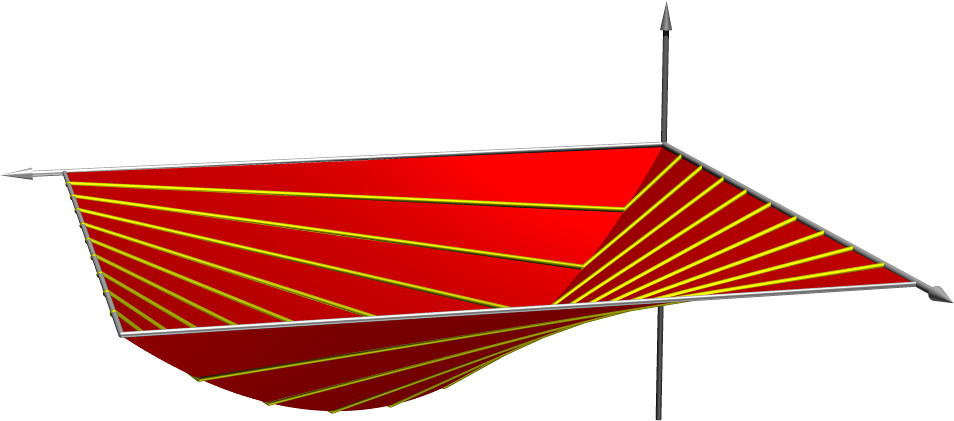
\includegraphics[width=\hsize]{../common/3d/green.jpg}
\end{center}
\caption{Darstellung der Greenschen Funktion $G(x,\xi)$
für das Problem $u''=f$ auf
dem Interval $[0,1]$ als Fläche über dem Quadrat $(x,\xi)\in[0,1]^2$.
Für jeden Wert von $\xi$ ist die partielle Funktion $x\mapsto G(x,\xi)$
eine Lösung der Differentialgleichung $u''=\delta_\xi$ zu den Randbedingungen
$u(0)=u(1)=0$.
\label{elliptisch:green3dflaeche}}
\end{figure}
\begin{figure}
\begin{center}
\includegraphics{../common/images/green-1.pdf}
\end{center}
\caption{Partielle Funktionen $x\mapsto G(x,\xi)$ der Greensche Funktion
des Problems $u''=f$ mit Randbedingungen $u(0)=u(1)=0$ für
verschiedene Werte von $\xi$.
\label{elliptisch:green1schar}}
\end{figure}

Die bis jetzt gefundenen Formeln für die Lösung $u(x)$
in Form eines Doppelintegrals haben noch
nicht die gewünschte Form eines einfachen Integrals.
Dies kann mit der Funktion $h$ korrigiert werden.
Die Funktion $x\mapsto h(x,\xi)=(x-\xi)\vartheta(x-\xi)$ hat die Randwerte
$0$ und $1-\xi$, also hat die Funktion
\[
G(x,\xi)
=
(x-\xi)\vartheta(x-\xi)-x(1-\xi)
=\begin{cases}
(x-\xi)+x(\xi-1)&\qquad x\le \xi \\
x(\xi-1)&\qquad x<\xi
\end{cases}
\]
die Randwerte $0$.
$G$ erfüllt
\[
\frac{\partial^2}{\partial x^2}G(x,\xi)=\delta(x-\xi)
\]
und
\[
G(0,\xi)=G(1,\xi)=0.
\]
Eine Lösung der Differentialgleichung lässt sich damit
als 
\[
u(x)=\int_0^1G(x,\xi)f(\xi)\,d\xi+a(1-x)+bx
\]
finden.

Der eindimensionale Fall zeigt also, dass man man zu dem Operator $D^2u=f$
mit der Funktion $G$ eine Inverse konstruieren kann.

Die Abbildungen \ref{elliptisch:green3dflaeche} und
\ref{elliptisch:green1schar} zeigen die Greensche Funktion $G(x,\xi)$.
Die partiellen Funktionen $x\mapsto G(x,\xi)$ sind jeweils Lösungen
des Problems $u''=\delta_\xi$ mit Randwerten $u(0)=u(1)=0$.
In den Abbildungen sind die partiellen Funktionen für eine Anzahl
von Werten $\xi$ hervorgehoben.

\begin{beispiel}
Die Differentialgleichung
\[
y''=\cos 3\pi x.
\]
hat die Lösung
\[
y(x)=-\frac1{9\pi^2}(\cos 3\pi x + 2x - 1),
\]
die man auch mit der Greenschen Funktion berechnen kann:
\[
y(x)=\int_0^1 G(x,\xi)\cos 3\pi\xi\,d\xi.
\]
In Abbildung
\ref{elliptisch:green-beispiele}
ist $f(x)=\cos 3\pi x$ durch eine Summe von einigen $\delta$-Distribution
approximiert worden (blau).
Die zugehörige Lösung ist jeweils rot eingezeichnet, sie hat
Knicke bei den $\delta$-Funktionen. 
Bei grösser werdender Zahl von $\delta$-Funktionen unterscheidet sich
das Integral $\int G(x,\xi)f(\xi)\,d\xi$ kaum mehr von der Lösung.
\begin{figure}
\begin{center}
\includegraphics[width=0.7\hsize]{../common/graphics/green-1.pdf}\\
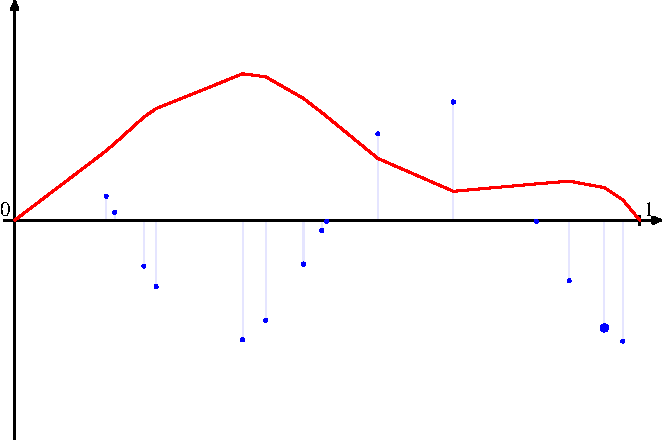
\includegraphics[width=0.7\hsize]{../common/graphics/green-324.pdf}\\
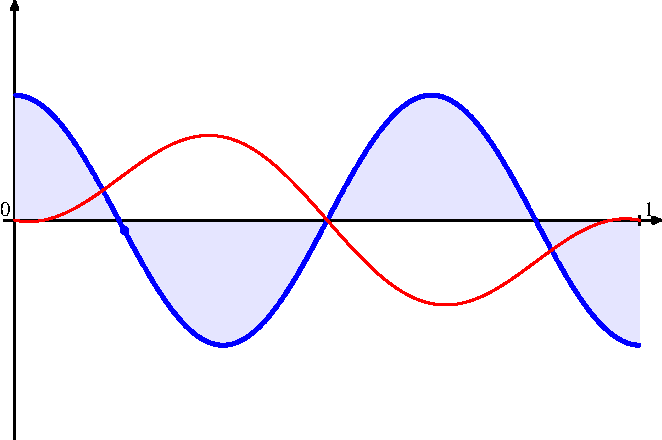
\includegraphics[width=0.7\hsize]{../common/graphics/green-1082.pdf}
\end{center}
\caption{Lösung (rot) von $y''=f$ für die Approximation der Funktion $f$
durch eine Summe von $\delta$-Distributionen (blau).
\label{elliptisch:green-beispiele}}
\end{figure}

Eine Animation der Berechnung der Lösung $y(x)$ mit der Greenschen
Funktion ist auch auf Youtube zu finden: \url{http://www.youtube.com/watch?v=Wpi7Gf7V2HY}
\end{beispiel}

